\subsection{Reasoning transfer in CLEVR-CoGenT}
\label{sec:reasoning-transfer-clevr}
In the following experiments, we used CoGent-A only.
Using the question categories defined by the authors, we organized training and testing splits with the goal of measuring whether mastering reasoning for one question category can help learning others.

\begin{figure}[htbp]
	\centering
	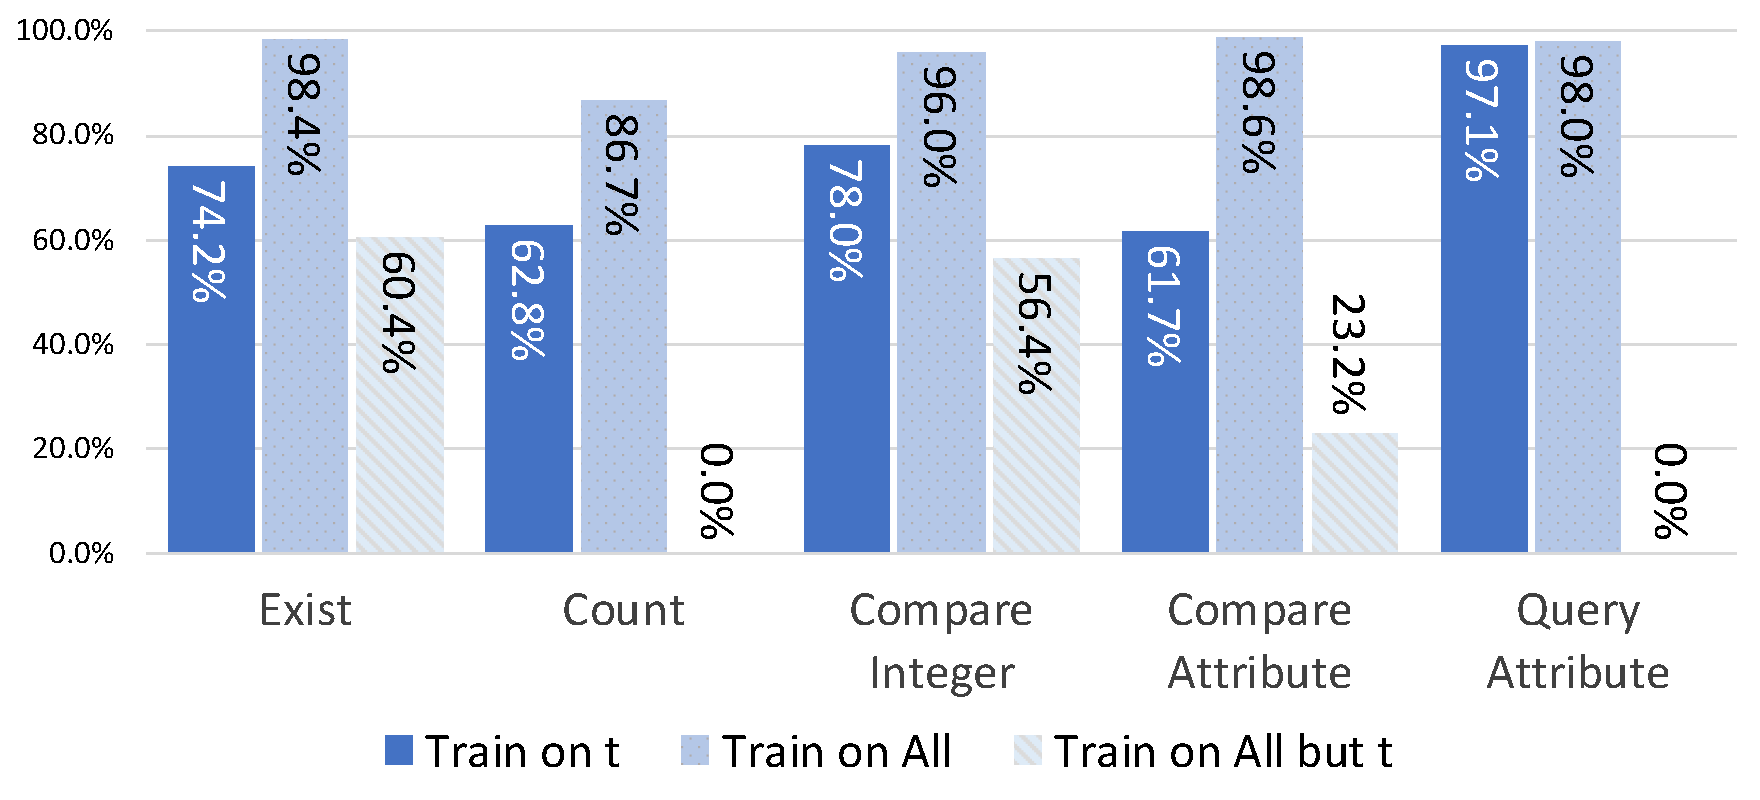
\includegraphics[width=0.8\textwidth]{../img/plots/cogent_reasoning_transfer.pdf}
	\caption{Accuracies of SAMNet when testing its reasoning transfer capabilities on the CoGenT-A variant.}
	\label{fig:cogent_reasoning_transfer}
\end{figure}

We first trained a single SAMNet instance on CoGenT-A and measured its accuracy on each of the question category $t$ separately.
Those results, indicated in \cref{fig:cogent_reasoning_transfer} as ``Train on All'', serve as baselines for the next two sets of experiments.

We next trained and tested 5 SAMNet instances, each on a single question category $t$ (``Train on $t$ only'').
We observe significant accuracy drops (from 18 up to almost 35 points) in all question categories, except for \textit{Query Attribute}.
We hypothesize \textit{Query Attribute} requires mastering visual grounding and recognizing object attributes, as opposed to the other groups which may not enforce it.
Thus, training on \textit{Query Attribute} helps others, whereas without any training on that particular group, SAMNet struggles developing such skill.

Finally, we trained 5 SAMNet instances as follows: for each category $t$, we trained a single instance on all categories but $t$, and tested its performance on
category $t$ only.
As expected, this setup appears challenging, causing severe performance drops, with accuracy on \textit{Count} and \textit{QueryAttribute} dropping to zero.
This stems from the non-overlapping labels spaces of \textit{Count} (digits 0 to 9) and \textit{QueryAttribute} (all attributes names) with the other groups (binary ``yes'' / ``no''). Thus, the model cannot predict these labels in a zero-shot transfer.


\subsection{Reasoning transfer in COG Canonical}
\label{sec:reasoning-transfer-cog}
In order to further investigate whether reasoning transfer is effective in leveraging information gained by training a question group at a higher level of the hierarchy, we also conducted a set of experiments using the Canonical variant of COG.
The order of the performed experiments is analogical to the one in the previous section.
The first column (\cref{fig:cog_reasoning_transfer}, ``Train on All'') is taken as a reference, i.e.
we train a single SAMNet instance on all questions and test on each of the five question groups from the hierarchy shown in~\cref{fig:question-groups}.
Note that these results are weighted averages of accuracies of our model on the Canonical variant (\cref{fig:samnet_cog_detailed}).

\begin{figure}[htbp]
	\centering
	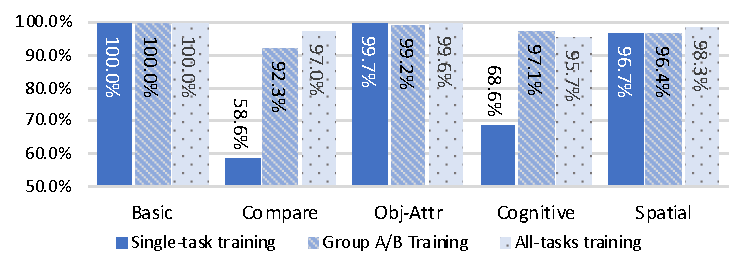
\includegraphics[width=0.8\textwidth]{../img/plots/cog_reasoning_transfer.pdf}
	\caption{Accuracies of SAMNet when testing its reasoning transfer capabilities on the Canonical variant of COG.}
	\label{fig:cog_reasoning_transfer}
\end{figure}

Next, we experimented with the ``Train on $t$ only'' setup, i.e. training and testing each of 5 SAMNet instances on a single question group $t$ (i.e. the leaves of the proposed hierarchy).
For \textit{Basic}, \textit{Spatial} and \textit{Obj-Attr}, the accuracy is matching the reference (``Train on All''), suggesting that each group contains sufficient information for developing all necessary skills.
Therefore, models trained on these groups may not benefit from any additional training on other question groups.
However, accuracy on \textit{Compary} and \textit{Cognitive} dropped, suggesting the contrary.

Therefore, we performed a final set of experiments (``Train on Group A/B''), where we trained two SAMNet instances: a) trained on all questions from \textit{Group A} and tested on each of the lowest groups below \textit{Group A}, i.e. \textit{Basic}, \textit{Obj-Attr} and \textit{Compare}, separately; b) trained on all questions from \textit{Group B} and tested separately on \textit{Spatial} and \textit{Cognitive} groups.
As expected, training on the other questions from \textit{Group A} enabled the model to significantly improve on the \textit{Compare} category (from 58.6\% to 92.3\%).
A similar improvement (from 68.8\% to 97.1\%) was observed in the second experiment, when trained on \textit{Group B} and tested on \textit{Cognitive}.
Moreover, the achieved accuracy is in fact higher by 1.4 point than the one achieved when training on all questions (95.7\%).
This suggests the model may have lacked capacity to master questions from all questions and that training on a smaller subset allowed better performance on this subset.
Finally, we can interestingly note for \textit{Obj-Attr} and \textit{Spatial} that training on the Group A/B does not appear to help. When comparing with ``Train on $t$ only'', we observe slight accuracy drops (around 0.3-0.5 point).
Understanding this phenomenon warrants further investigations on the dependencies between the reasoning required by the particular questions and the transferred reasoning.
